
\section{Ejercicio 1 Opcional}
El alumno/a debe ser capaz de presentar un MV con la configuración descrita en este apartado. La configuración debe ser permanente, es decir, en todo caso, tras reiniciar el equipo, la configuración será la esperada.
Para validar la configuración de red, el alumno/a debe ser capaz de:
\begin{itemize}
    \item Hacer ping desde el equipo anfitrión a la MV y viceversa.
    \item Hacer ping desde la MV a cualquier equipo accesible públicamente en Internet por FQHN o IP.
    \item Conectar por ssh desde el equipo anfitrión a la MV .
\end{itemize}

\subsection{Solución}
Una vez que hayamos instalado el SO que se nos pide correctamente. Debemos de realizar una serie de ajustes previos:
\begin{itemize}
    \item Añadir nuestro usuario, para ello debemos de ejecutar lo siguientes comandos (iniciando como usuario root):
    \begin{itemize}
        \item \texttt{sudo useradd nombre\_de\_usuario}        
        \item \texttt{sudo passwd nombre\_de\_usuario}
        \item \texttt{sudo usermod -aG wheel nombre\_de\_usuario} para que pueda usar el comando sudo.
    \end{itemize}
\end{itemize}

\begin{itemize}
    \item Configurar la red NAT y una de tipo Host-Only, para ello en Herramientas en la VM debemos seleccionar la opción de Red y añadir una nueva interfaz de red de tipo Host-Only, y paso seguido configurar la red NAT (ver Figura 1 y 2 )
    \item Comprobar que el servicio SSH está instalado, por defecto se suele instalar, para asegurarnos debemos de ejecutar el comando \texttt{sudo systemctl status ssh}. En el caso de que no venga instalado debemos de ejecutar el comando \texttt{sudo dnf install -y openssh-server openssh-clients}\footnote{Incluimos clients para añadir el servicio de cliente.} (Ver Figura 5).
    \item Cambiar la variable PS1 como se nos pedía, para ello debemos de editar el fichero de bashrc y exportar la variable PS1 con el valor que se nos pedía:
    \begin{itemize}
        \item \texttt{PS1='\textbackslash u@\textbackslash h:\textbackslash t:\textbackslash w\textbackslash\$ '} (Ver Figura 5), donde:
        \begin{itemize}
            \item \texttt{\textbackslash u}: Nombre del usuario actual.
            \item \texttt{\textbackslash h}: Nombre del hostname (nombre del sistema).
            \item \texttt{\textbackslash t}: Hora actual en formato de 24 horas (HH:MM:SS).
            \item \texttt{\textbackslash w}: Directorio de trabajo actual.
            \item \texttt{\$}: Símbolo del prompt, que será \$ para un usuario normal y \# para root.
        \end{itemize}
    \end{itemize}
\end{itemize}

\begin{figure}[htbp]
    \centering
    \begin{minipage}[b]{0.45\textwidth}
        \centering
        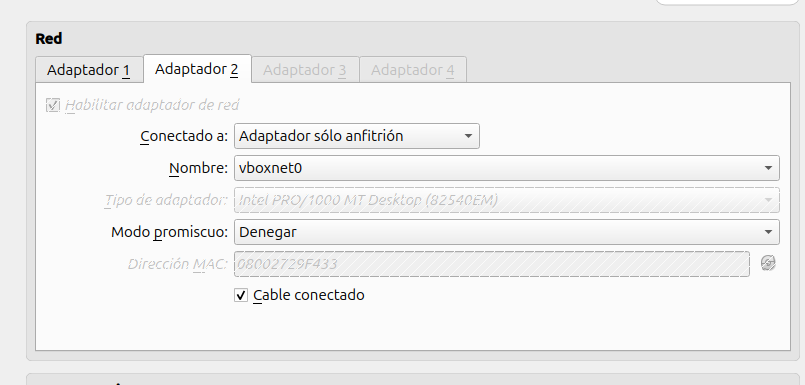
\includegraphics[width=\textwidth]{images/Bloque1/adaptador2.png}
        \caption{Configuración de la red NAT y Host-Only}
    \end{minipage}
    \hfill
    \begin{minipage}[b]{0.45\textwidth}
        \centering
        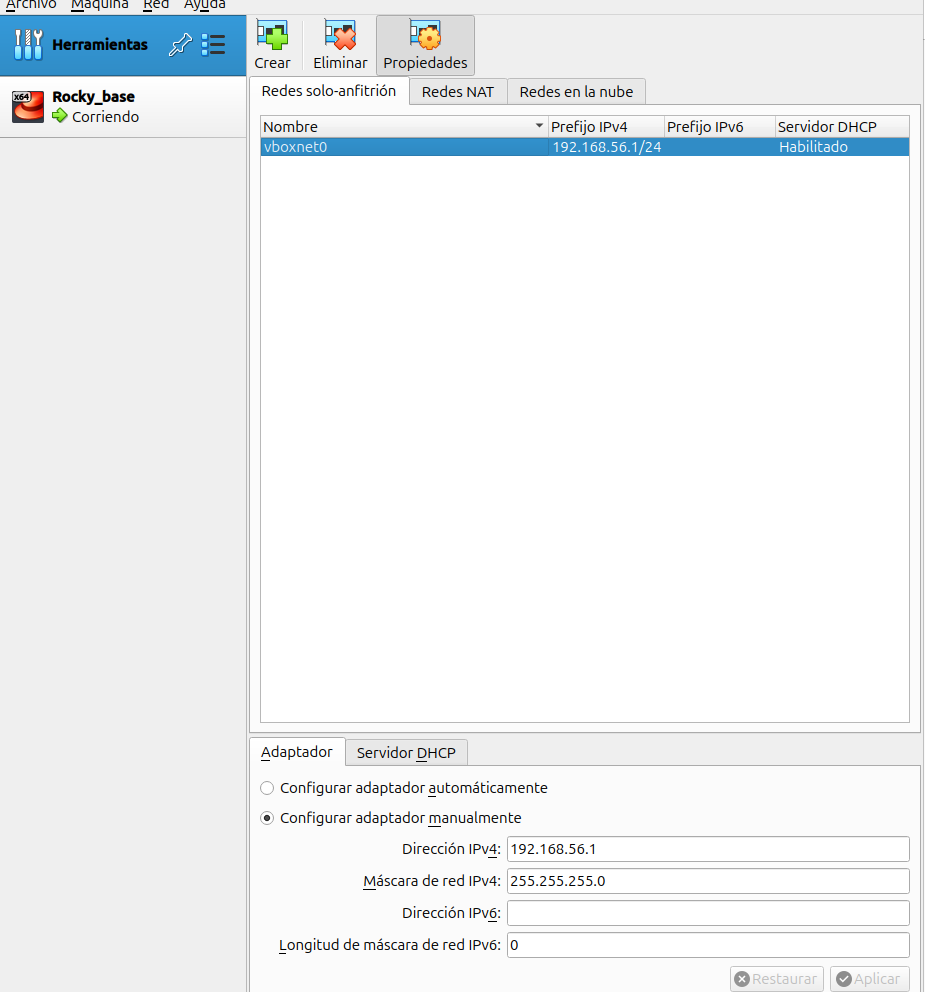
\includegraphics[width=\textwidth]{images/Bloque1/vbox.png}
        \caption{Configuración de VirtualBox para la red de Host-Only}
    \end{minipage}
\end{figure}

Además se nos pide que la Ip de Host Only sea estática, para ello vamos a asegurarnos usando la herramienta \textit{nmtui}, en la que vamos a ver si es estática o no la ip. Como podemos ver en la siguiente imagen esta configurada como ip automática, que viene siendo lo mismo que dinámica por lo que debemos de cambiarlo a manual para poder configurar la ip estática. (Ver Figura 3 y 4). Para ver que efectivamente la ip cambió, podemos verlo en la Figura 5.
\begin{figure}[htbp]
    \centering
    \begin{minipage}[b]{0.45\textwidth}
        \centering
        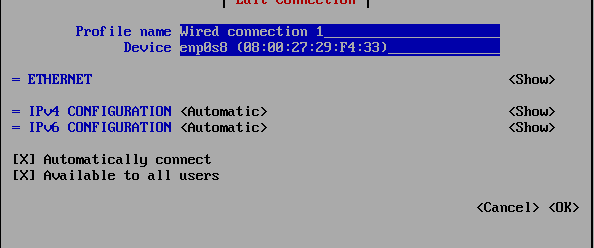
\includegraphics[width=\textwidth]{images/Bloque1/nmtui1.png}
        \caption{Con nmtui vemos que es dinámica}
    \end{minipage}
    \hfill
    \begin{minipage}[b]{0.45\textwidth}
        \centering
        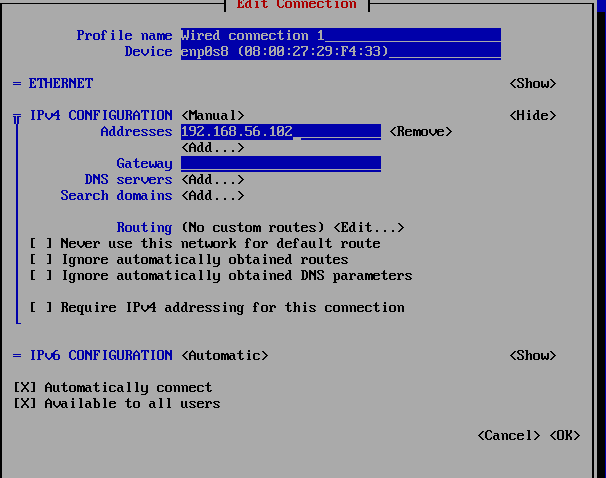
\includegraphics[width=\textwidth]{images/Bloque1/nmtui_2.png}
        \caption{Cambiamos a manual y asignamos una ip estática válida}
    \end{minipage}
\end{figure}



\begin{figure}
    \centering
    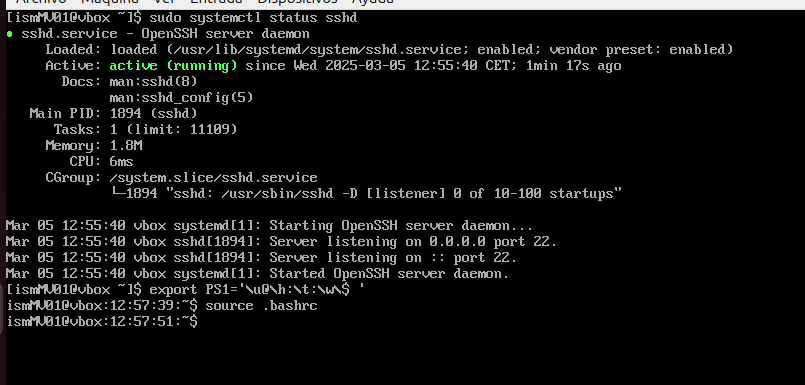
\includegraphics[width=0.8\textwidth]{images/Bloque1/sshd_PS1.png}
    \caption{Sshd y variable PS1}
\end{figure}

\begin{figure}
    \centering
    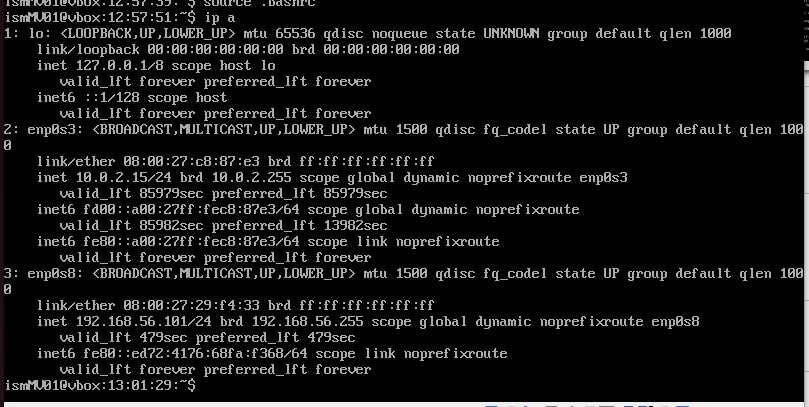
\includegraphics[width=0.8\textwidth]{images/Bloque1/resultado_ipa.png}
    \caption{Resultado de ip a}
\end{figure}

Una vez hayamos cambiado la ip estática, debemos de verificar que efectivamente se ha cambiado y para ello usamos el comando \texttt{ip a} y vemos que efectivamente se ha cambiado la ip a la que hemos asignado. (Ver Figura 7).

\begin{figure}
    \centering
    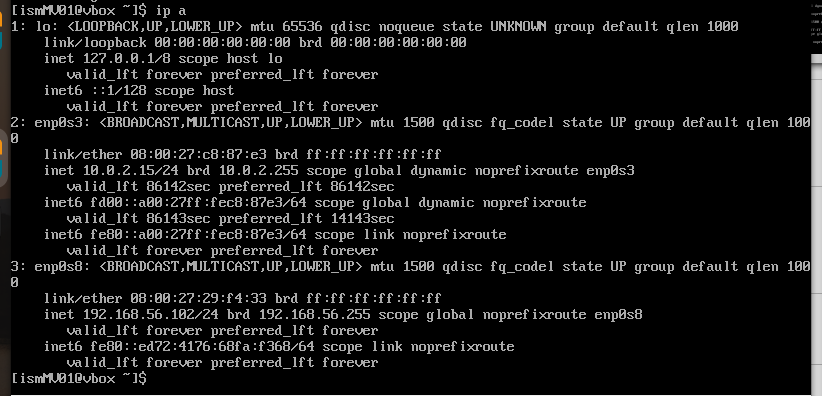
\includegraphics[width=0.8\textwidth]{images/Bloque1/ping2.png}
    \caption{Resultado de ip a para verificar el cambio de ip}
\end{figure}

Llegado a este punto vamos a realizar un ping a la máquina anfitriona y viceversa, para ello usamos el comando \texttt{ping -c <número de pings> ip\_de\_la\_maquina} y vemos que efectivamente hay conexión entre ambas máquinas. (Ver Figura 8, 9 y 10). Además, vemos que gracias al \textit{NAT} podemos hacer ping a cualquier máquina accesible en internet\footnote{Cabe destacar que durante el desarrollo de la actividad, surgían algunas problemas con NetworkManager, polkiy y DBus, pero se solucionaban al reiniciarlos o bien reinstalarlos}. (Ver Figura 11).

\begin{figure}[htbp]
    \centering
    \begin{minipage}[b]{0.45\textwidth}
        \centering
        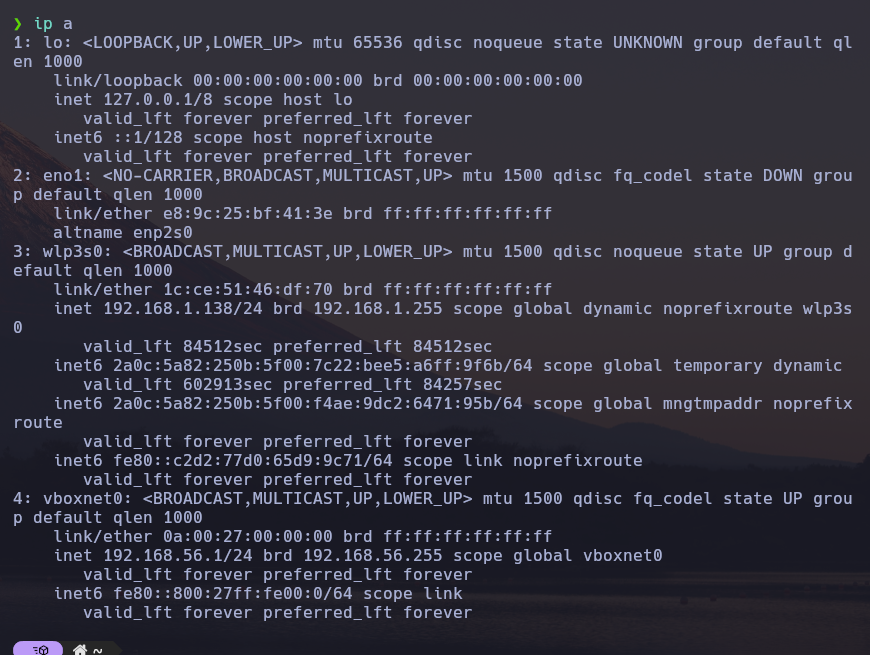
\includegraphics[width=\textwidth]{images/Bloque1/ip_a_host.png}
        \caption{Resultado del comando de \textit{ip a } en la máquina anfitriona para ver la ip}
    \end{minipage}
    \hfill
    \begin{minipage}[b]{0.45\textwidth}
        \centering
        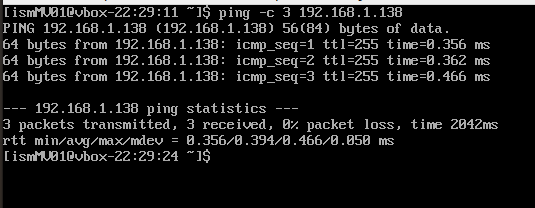
\includegraphics[width=\textwidth]{images/Bloque1/ping_a_anfitriona.png}
        \caption{Ping a la máquina anfitriona}
    \end{minipage}
\end{figure}


\begin{figure}[htbp]
    \centering
    \begin{minipage}[b]{0.45\textwidth}
        \centering
        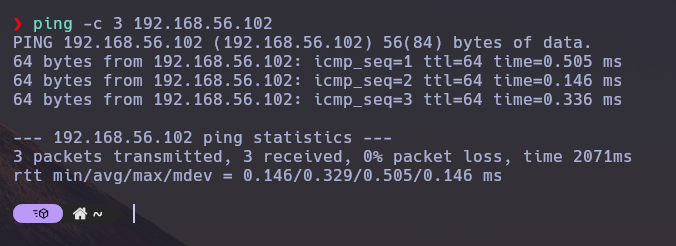
\includegraphics[width=\textwidth]{images/Bloque1/ping_anf_a_mv.png}
        \caption{Ping de la máquina anfitriona a la máquina virtual}
    \end{minipage}
    \hfill
    \begin{minipage}[b]{0.45\textwidth}
        \centering
        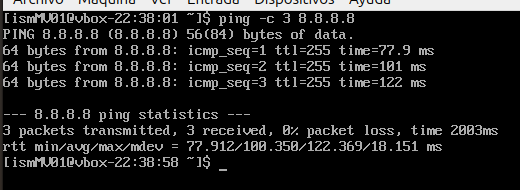
\includegraphics[width=\textwidth]{images/Bloque1/ping_fuera.png}
        \caption{Ping a un servidor público (Google)}
    \end{minipage}
\end{figure}


En cuanto al servicio ssh, debemos de ver el estado del servicio sshd con el comando \texttt{sudo systemctl status sshd} y vemos que esta corriendo. En este punto desde el anfitrión podemos introducirt la línea de comando \texttt{ssh ismMV01@192.168.56.102} y vemos que efectivamente todo funciona correctamente. (Ver Figura 12 y 13).






\begin{figure}[htbp]
    \centering
    \begin{minipage}[b]{0.45\textwidth}
        \centering
        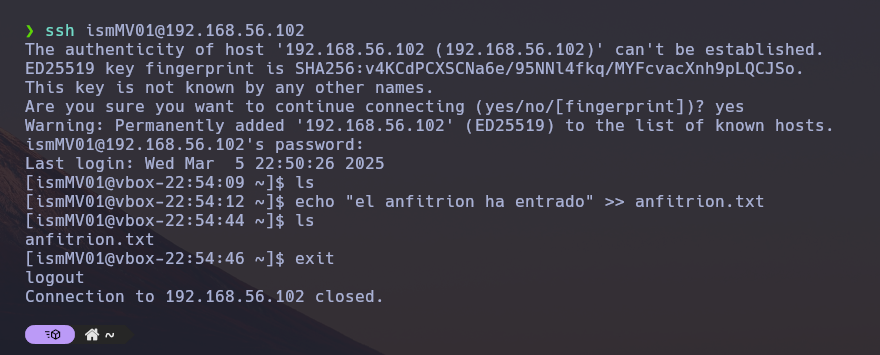
\includegraphics[width=\textwidth]{images/Bloque1/ssh1.png}
        \caption{Ssh en la máquina anfitriona y creación de un archivo en la MV}
    \end{minipage}
    \hfill
    \begin{minipage}[b]{0.45\textwidth}
        \centering
        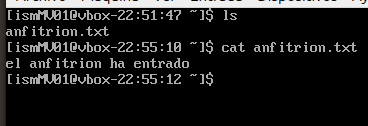
\includegraphics[width=\textwidth]{images/Bloque1/ssh2.png}
        \caption{Ver el contenido del archivo creado en la MV desde el anfitrión}
    \end{minipage}
\end{figure}

\section{Servidor con LVM + RAID}

\subsection{Aspectos clave de LVM}

Para gestionar eficazmente el \textit{Logical Volume Manager} (LVM), es fundamental comprender los siguientes componentes y conceptos:

\subsubsection{Componentes de la arquitectura de almacenamiento}

\begin{itemize}
  \item \textbf{Physical Volume (PV)}: Representa los dispositivos de almacenamiento físico, como discos duros o particiones, que se incorporan al sistema LVM.
  \item \textbf{Volume Group (VG)}: Es una agrupación de uno o más PVs que forman un pool de almacenamiento, del cual se pueden asignar espacios para crear volúmenes lógicos.
  \item \textbf{Logical Volume (LV)}: Son volúmenes virtuales creados dentro de un VG. Los LVs se utilizan como si fueran particiones de disco tradicionales, permitiendo la creación de sistemas de archivos o la asignación directa a aplicaciones.
\end{itemize}

\subsubsection{Gestión de almacenamiento con diferentes características físicas}

LVM ofrece flexibilidad para manejar dispositivos de almacenamiento con diversas características físicas:

\begin{itemize}
  \item \textbf{HDD y SSD}: Se pueden combinar en un mismo VG, permitiendo equilibrar rendimiento y capacidad según las necesidades.
  \item \textbf{RAID}: LVM puede trabajar sobre dispositivos RAID, proporcionando una capa adicional de gestión y flexibilidad sobre la configuración RAID existente.
\end{itemize}

\subsubsection{Etiquetado y correspondencia con los archivos de dispositivo}

Cada componente en LVM tiene una nomenclatura específica y se asocia a archivos de dispositivo en el sistema:

\begin{itemize}
  \item \textbf{Physical Volumes}: Corresponden a dispositivos físicos, como \texttt{/dev/sda1}, \texttt{/dev/sdb1}, etc.
  \item \textbf{Volume Groups}: Se nombran según la convención establecida por el administrador, por ejemplo, \texttt{vg\_datos}.
  \item \textbf{Logical Volumes}: Se nombran dentro de su VG correspondiente, como \texttt{/dev/vg\_datos/lv\_backup}, donde \texttt{lv\_backup} es el nombre del LV.
\end{itemize}

\subsubsection{Comandos de LVM para la gestión de componentes}

LVM proporciona una serie de comandos para administrar sus componentes:

\begin{itemize}
  \item \texttt{pvcreate}: Inicializa un dispositivo físico como PV.
  \item \texttt{vgcreate}: Crea un VG a partir de uno o más PVs.
  \item \texttt{lvcreate}: Crea un LV dentro de un VG.
  \item \texttt{pvs}, \texttt{vgs}, \texttt{lvs}: Muestran información sobre PVs, VGs y LVs respectivamente.
  \item \texttt{pvremove}, \texttt{vgremove}, \texttt{lvremove}: Eliminan PVs, VGs y LVs respectivamente.
\end{itemize}

Estos comandos permiten una gestión eficiente y flexible del almacenamiento en sistemas que utilizan LVM.

\subsection{Niveles de RAID: 0, 1 y 5}

Redundant Array of Independent Disks (RAID) es una tecnología que permite combinar múltiples dispositivos de almacenamiento en una unidad lógica para mejorar el rendimiento, la redundancia o ambos. A continuación, se detallan los niveles de RAID 0, 1 y 5, sus ventajas, desventajas y su administración en sistemas Linux utilizando la herramienta de línea de comandos \texttt{mdadm}.

\subsubsection{RAID 0}

RAID 0, conocido como \textit{striping}, distribuye los datos de manera equitativa entre dos o más discos sin información de paridad ni redundancia.

\begin{itemize}
  \item \textbf{Ventajas}:
    \begin{itemize}
      \item Mayor rendimiento en lectura y escritura debido a la distribución de datos entre los discos.
      \item Uso completo de la capacidad de almacenamiento total, ya que no se reserva espacio para paridad o duplicación.
    \end{itemize}
  \item \textbf{Desventajas}:
    \begin{itemize}
      \item Ausencia de redundancia; la falla de un solo disco resulta en la pérdida total de los datos.
    \end{itemize}
\end{itemize}

\subsubsection{RAID 1}

RAID 1, o \textit{mirroring}, duplica los datos en dos o más discos, creando copias idénticas en cada uno.

\begin{itemize}
  \item \textbf{Ventajas}:
    \begin{itemize}
      \item Alta redundancia; los datos permanecen intactos incluso si uno de los discos falla.
      \item Mejora en la velocidad de lectura, ya que los datos pueden leerse desde cualquiera de los discos.
    \end{itemize}
  \item \textbf{Desventajas}:
    \begin{itemize}
      \item Capacidad de almacenamiento efectiva reducida al 50\% del total, ya que los datos se duplican.
    \end{itemize}
\end{itemize}

\subsubsection{RAID 5}

RAID 5 combina rendimiento y redundancia distribuyendo los datos y la paridad entre tres o más discos.

\begin{itemize}
  \item \textbf{Ventajas}:
    \begin{itemize}
      \item Proporciona tolerancia a fallos; si un disco falla, los datos pueden recuperarse con la información de paridad.
      \item Mejor aprovechamiento del almacenamiento comparado con RAID 1, ya que solo se utiliza una fracción del espacio para la paridad.
    \end{itemize}
  \item \textbf{Desventajas}:
    \begin{itemize}
      \item Rendimiento de escritura inferior al de RAID 0 debido al cálculo de la paridad.
      \item En caso de falla de un disco, la reconstrucción puede ser lenta y afectar el rendimiento.
    \end{itemize}
\end{itemize}

\subsubsection{Administración de RAID en Linux con mdadm}

La herramienta \texttt{mdadm} permite gestionar arreglos RAID en Linux. A continuación, se presentan comandos esenciales:

\begin{itemize}
  \item Crear un RAID 0 con dos discos:
    \begin{lstlisting}
    mdadm --create --verbose /dev/md0 --level=0 --raid-devices=2 /dev/sdX /dev/sdY
    \end{lstlisting}
  \item Crear un RAID 1 con dos discos:
    \begin{lstlisting}
    mdadm --create --verbose /dev/md0 --level=1 --raid-devices=2 /dev/sdX /dev/sdY
    \end{lstlisting}
  \item Crear un RAID 5 con tres discos:
    \begin{lstlisting}
    mdadm --create --verbose /dev/md0 --level=5 --raid-devices=3 /dev/sdX /dev/sdY /dev/sdZ
    \end{lstlisting}
  \item Verificar el estado del RAID:
    \begin{lstlisting}
    cat /proc/mdstat
    \end{lstlisting}
  \item Detener un RAID:
    \begin{lstlisting}
    mdadm --stop /dev/md0
    \end{lstlisting}
\end{itemize}

\subsection{Aspectos clave para la administración de servidores Linux}

Para implementar eficazmente soluciones en servidores Linux, es esencial comprender y manejar los siguientes aspectos:

\subsubsection{Modos de ejecución y modo de mantenimiento en un servidor Linux}

Los sistemas Linux operan en diferentes niveles de ejecución o \textit{runlevels}, que determinan los servicios y procesos que se ejecutan. Con la adopción de \textit{systemd}, estos niveles se denominan \textit{targets}. El modo de mantenimiento, conocido como \textit{rescue.target} o \textit{emergency.target}, es crucial para tareas de recuperación y administración del sistema. Para cambiar al modo de mantenimiento, se puede utilizar el siguiente comando:

\begin{lstlisting}
sudo systemctl isolate rescue.target
\end{lstlisting}

Para volver al modo multiusuario estándar:

\begin{lstlisting}
sudo systemctl isolate multi-user.target
\end{lstlisting}

\subsubsection{Estructura estándar del sistema de archivos en Linux}

La estructura de directorios en Linux sigue el estándar de jerarquía de sistemas de archivos (\textit{Filesystem Hierarchy Standard - FHS}). Algunos directorios principales incluyen:

\begin{itemize}
  \item \textbf{/}: Directorio raíz que contiene todos los demás directorios.
  \item \textbf{/bin}: Ejecutables esenciales para todos los usuarios.
  \item \textbf{/etc}: Archivos de configuración del sistema.
  \item \textbf{/home}: Directorios personales de los usuarios.
  \item \textbf{/var}: Datos variables como registros y colas de impresión.
\end{itemize}

\subsubsection{Sistemas de archivos comunes en Linux}

Linux soporta diversos sistemas de archivos. Algunos de los más comunes son:

\begin{itemize}
  \item \textbf{ext4}: Sistema de archivos por defecto en muchas distribuciones, conocido por su estabilidad y rendimiento.
  \item \textbf{XFS}: Adecuado para manejar grandes volúmenes de datos y archivos de gran tamaño.
  \item \textbf{Btrfs}: Ofrece características avanzadas como instantáneas (\textit{snapshots}) y compresión.
\end{itemize}

\subsubsection{Montaje y desmontaje de volúmenes}

El montaje de sistemas de archivos permite acceder a dispositivos de almacenamiento. Para montar un dispositivo:

\begin{lstlisting}
sudo mount /dev/sdX1 /mnt/punto_de_montaje
\end{lstlisting}

Para desmontarlo:

\begin{lstlisting}
sudo umount /mnt/punto_de_montaje
\end{lstlisting}

Las configuraciones de montaje persistentes se definen en el archivo \texttt{/etc/fstab}.

\subsubsection{Comandos básicos para la gestión de archivos}

La administración de archivos en Linux se realiza mediante comandos de línea. Algunos comandos fundamentales incluyen:

\begin{itemize}
  \item \texttt{cp}: Copiar archivos o directorios.
    \begin{lstlisting}
    cp origen destino
    \end{lstlisting}
  \item \texttt{mv}: Mover o renombrar archivos o directorios.
    \begin{lstlisting}
    mv origen destino
    \end{lstlisting}
  \item \texttt{rm}: Eliminar archivos.
    \begin{lstlisting}
    rm archivo
    \end{lstlisting}
  \item \texttt{mkdir}: Crear un nuevo directorio.
    \begin{lstlisting}
    mkdir nombre_del_directorio
    \end{lstlisting}
  \item \texttt{ls}: Listar el contenido de un directorio.
    \begin{lstlisting}
    ls ruta_del_directorio
    \end{lstlisting}
  \item \texttt{cat}: Mostrar el contenido de un archivo.
    \begin{lstlisting}
    cat archivo
    \end{lstlisting}
  \item \texttt{nano} o \texttt{vim}: Editores de texto para modificar archivos desde la terminal.
    \begin{lstlisting}
    nano archivo
    \end{lstlisting}
\end{itemize}

Estos comandos son esenciales para la gestión diaria de archivos y directorios en un entorno Linux.
Estos se deben de haber estudiado en asignaturas anteriores como Sistemas Operativos.

\subsection{Ejercicio Opcional}

Partiendo de un servidor básico configurado de acuerdo al apartado 2, el alumno/a deberá
afrontar el caso práctico descrito a continuación:

Se desea instalar un servicio de gestión documental en el servidor. Se espera que este servicio
precise de una cantidad espacio de almacenamiento creciente con el tiempo, pudiendo llegar a
ser considerable.

Por otro lado, el contenido será crítico, por lo que se desea proporcionar
algún mecanismo de respaldo ante fallos en el dispositivo de almacenamiento.

El alumno/a debe diseñar los cambios en el sistema de almacenamiento e implementarlo
empleando prácticas adecuadas de administración que garanticen la conservación de la
información en el sistema y procuren la máxima disponibilidad del servicio.

\subsubsection{Solución}

Para la resolución de este ejercicio vamos a seguir lo realizado en clase. (Ver apuntes de clase correspondientes a la sección de LVM+RAID).



